\section{Linear Equations with Constant Equations}

\subsection{Auxiliary Equation}

Linear homogeneous DE with constant coefficients can be expressed as

\begin{equation}
    a_{0} \frac{d^{n} y}{d x^{n}}+a_{1} \frac{d^{n-1} y}{d x^{n-1}}+\cdots+a_{n-1} \frac{d y}{d x}+a_{n} y=0
\end{equation}

Can be written in the form

\begin{equation}
    f(D)y=0
\end{equation}

where $f(D)$ is a linear differential operator. If the algebraic eqn $f(m)=0$
then we know $f(D)e^{mx}=0\implies y=e^{mx}$ is a solution to the form above.
$f(m)=0$ is the auxiliary equation associated with the DE.
Since the DE is of order $n$, the auxiliary equation is of degree $n$ with
roots $m_1,\ldots,m_n$.

Thus we have $n$ solutions $y_1=\exp(m_1x),\ldots,y_n=\exp(m_nx)$ assuming
the roots are \textbf{real} and \textbf{distinct} are then \textbf{linearly independent}.
The general solution is thus

\begin{equation}
    y=c_1\exp(m_1x)+\cdots+c_n\exp(m_nx)
\end{equation}

with arbitrary constants $c_1,\ldots,c_n$.

\subsubsection{Derivation}

We can say that $y^{(k)}$ is the $k$th derivative of $y$, so say the general form is

$$
a_ny^{(n)}+a_{n-1}y^{(n-1)}+\cdots+a_1y^\prime +a_0y=0
$$

If we take $y=e^{rx}$, then observe $y^{(n)}=r^ne^{rx}$. So rewrite the general form as

\begin{align*}
    a_nr^ne^{rx}+a_{n-1}r^{n-1}e^{rx}+\cdots+a_1re^{rx}+a_0e^{rx}&=0\\
    a_nr^n+a_{n-1}r^{n-1}+\cdots+a_1r+a_0&=0
\end{align*}

Solving for the roots $r$ in this characteristic equation helps us obtain the general solution.

\subsection{Auxiliary Equation Repeated Roots}

Need method for obtaining $n$ linearly independent solutions for $n$ equal roots of auxiliary equation.
Suppose auxiliary equation $f(m)=0$ has $n$ roots $m_1=m_2=\cdots=m_n=b$.
Thus, the operator function $f(D)$ has a factor $(D-b)^n$. Want to find $n$ linearly independent $y$ for which $(D-b)^ny=0$.
Use the substitution $y_k=x^ke^{bx}$ such that

\begin{equation}
    (D-b)^n(x^ke^{bx})=0,\;k=0,1,2,\ldots,n-1
\end{equation}

The functions $y_k=x^ke^{bx}$ are linearly independent because the respective powers $x^0,\ldots,x^k$ are linearly independent.
So the general solution takes form

\begin{equation}
    y=c_1e^{bx}+c_2xe^{bx}+\cdots+c_nx^{n-1}e^{bx}
\end{equation}

\subsection{Complex roots for the auxiliary equation}

Complex roots typically come in conjugate pairs of the form $a\pm bi$.
So using the general form of the auxiliary solution and the Euler identity $e^{i\theta}=\sin\theta + i\cos\theta$ and the fact that $\cos(-x)=\cos x, \sin(-x)=-\sin x$, we find that

\begin{align}
    y_1&=c_1e^{(a+bi)x}=c_1e^{ax}e^{bxi}=c_1e^{ax}\left(\sin bx + i\cos bx\right)\\
    y_2&=c_2e^{(a-bi)x}=c_2e^{ax}e^{-bxi}=c_2e^{ax}\left(-\sin bx + i\cos bx\right)\\
    y_1+y_2&=c_1e^{ax}\left(\sin bx + i\cos bx\right)+c_2e^{ax}\left(-\sin bx + i\cos bx\right)\\
    &=e^{ax}(c_1-c_2)\sin bx + e^{ax}(c_1+c_2)i\cos bx\\
    &=c_3e^{ax}\sin bx + c_4e^{ax}\cos bx
\end{align}

\subsection{Linear Independence}

Linear independence of two functions $f_1,f_2$ is calculated with a determinant called the Wronskian $W(f_1,f_2)$.

\begin{equation}
    W(f_1,f_2)=\left|\begin{matrix}f_1&f_2\\f_1\,'&f_2\,'\end{matrix}\right|
\end{equation}

Let $f_1,f_2$ be differentiable on $[a,b]$. if $W(f_1,f_2)(t_0)\neq 0$ for some $t\in [a,b]$ then $f_1,f_2$ are linearly independent on $[a,b]$.
If they are linearly dependent, $W(f_1,f_2)(t)=0\;\forall t$.

\subsection{Review of rational roots, synthetic division}

For rational roots test, take factors of constant coeff. $c$ divided by factors of
leading coefficient $a$ to get possible roots.

\subsection{Undetermined Coefficients}

Can apply to the general form of a problem where

\begin{equation}
    f(D)y=R(x)
\end{equation}

Roots of the aux. eqn $f(m)=0$ are $m=m_1,\ldots,m_n$.
General sol'n is $y=y_c+y_p$. We suppose that $R(x)$ is a particular solution of some equation equation $g(D)R=0$.
This equation has its own set of roots $m'=m_1',\ldots,m_n'$, which you can find from inspection of $R$.

So the DE $g(D)R=0$, or

\begin{equation}
    g(D)f(D)y=0
\end{equation}

has the roots from $m,m'$. So the solution is of the form $y=y_c+y_q$ where $y_q$ satisfied $g(D)=0$.
We now observe that a particular solution of the original DE $f(D)y=R(x)$ must also satisfy the above DE.
Thus,

\begin{equation}
    f(D)(y_c+y_q)=R(x)
\end{equation}

Since $f(D)y_c=0$,

\begin{equation}
    f(D)y_q=R(x)
\end{equation}

So we can find coefficients to satisfy $y_q=y_p$.
Method can only be applied when $R(x)$ is a solution to homogeneous linear DE with constant coefficients.

\subsection{Variation of Parameters}

We start with the general equation

\begin{equation}
    ay''+by'+cy=g(x)
\end{equation}

First, find complementary solution $y_c$ from $y=y_p+y_c$. This is simply the solution of the homogeneous equation

\begin{equation}
    ay''+by'+cy=0
\end{equation}

Then, find the particular solution $y_p=u_1y_1+u_2y_2$ using Cramer's rule. Define 

\begin{equation}
W=
\begin{array}{|cc|}
    y_1&y_2\\
    y_1'&y_2'
\end{array}\;\;
W_1=\begin{array}{|cc|}
    0&y_2\\
    g(x)'&y_2'
\end{array}\;\;
W_2=\begin{array}{|cc|}
    y_1&0\\
    y_1'&g(x)'
\end{array}
\end{equation}

When we set up the matrix-vector equation $\mathrm{A}\mathbf{x}=\mathbf{b}$, it corresponds to the following:

\begin{equation}
    \begin{bmatrix}
        y_1 & y_2\\
        y_1' & y_2'
    \end{bmatrix}
    \begin{bmatrix}
        u_1\\u_2
    \end{bmatrix}
    =\begin{bmatrix}
        0\\g(x)
    \end{bmatrix}
\end{equation}

Following Cramer's rule, to find the solutions $1,\ldots,n$, we create $A_n$ by replacing the $n$th row of $A$ with $b$.

Strategy is to find $u_1', u_2'$ then integrate to find the coefficients and thus the eventual solution.

\begin{eqnarray}
    u_1'=\frac{W_1}{W}\\
    u_2'=\frac{W_2}{W}
\end{eqnarray}

\subsection{Reduction of Order}

Method is derived from the general 2nd order linear DE. Useful when $y_p$ does not correspond to a template solution class.

\begin{equation}
    y''+py'+qy=R\label{original}
\end{equation}

Assume there exists a solution $y=y_1$ of the homogeneous equation (e.g. can pick a solution from $y_c$).

\begin{eqnarray}
    y''+py"+qy=0
\end{eqnarray}

We then introduce a dependent variable from $y=y_1v$ as $v$. It follows that

\begin{eqnarray}
    y'=y_1v'+y_1'v\\
    y''=y_1v''+2y_1'v'+y_1''v
\end{eqnarray}

So substituting into \ref{original}, we get

\begin{equation}
    y_{1} v^{\prime \prime}+2 y_{1}^{\prime} v^{\prime}+y_{1}^{\prime \prime} v+p y_{1} v^{\prime}+p y_{1}^{\prime} v+q y_{1} v=R
\end{equation}

This rearranges to

\begin{equation}
    y_{1} v^{\prime \prime}+\left(2 y_{1}^{\prime}+p y_{1}\right) v^{\prime}+\left(y_{1}^{\prime \prime}+p y_{1}^{\prime}+q y_{1}\right) v=R .
\end{equation}

We use the definition of the homogeneous equation, since $y=y_1$ is a solution of the above.

\begin{equation}
    y_1v''+(2y_1'+py_1)v'=R
\end{equation}

If we let $v'=w$ and solve for $w$, then integrate, it is simply a first order problem with integrating factor

\begin{equation}
    k(x)=\exp{\int \frac{2y_1'+py_1}{y_1} dx}
\end{equation}

Another way to simplify this problem is to derive the general form of the reduction of order coefficient $v$,
from which solution $y=vy_1$ follows trivially.

\subsection{Spring Oscillation}

\begin{figure}[H]
    \centering
    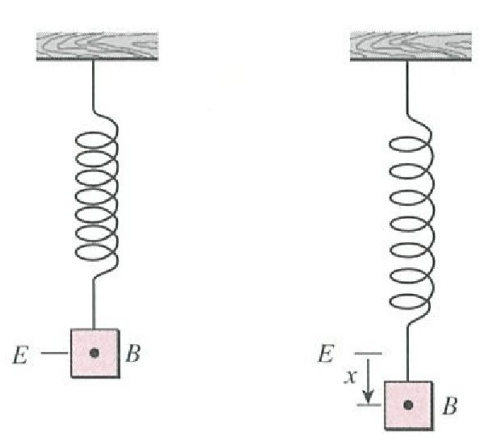
\includegraphics[scale=0.8]{figures/Screen Shot 2021-12-05 at 5.16.10 PM.png}
    \caption{Spring at equilibrium and stretched positions}
\end{figure}

By setting $E$ as the gravitational equilibrium position with some mass $B$, can avoid consideration of the original length of the spring.
Mass of the spring comes from $w=mg\implies m = \frac{w}{g}$. In addition to the restoring force which causes the block $B$ to accelerate, there is a
damping force proportional to velocity that acts in opposition to the direction of motion. Taking downwards to be conventionally positive, net force equation is

\begin{equation}
    \frac{w}{g}\ddot x=-kx-b\dot x
\end{equation}

This is better illustrated as follows (for now $F=0$)

\begin{figure}[H]
    \centering
    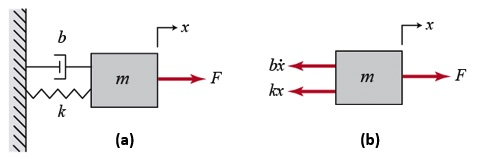
\includegraphics[scale=0.6]{figures/a-Mass-Spring-Damper-System-b-free-body-diagram.jpg}
    \caption{Damped spring oscillator}
\end{figure}

So the form of the DE becomes

\begin{equation}
    \frac{w}{g}\ddot x+b\dot x+kx=0
\end{equation}

This is a second order homogeneous equation. If we impose another driving force (as shown above, but with $F$ as a function of $t$) that acts on the mass DE becomes

\begin{equation}
    \frac{w}{g}\ddot x+b\dot x+kx=F(t)
\end{equation}

The initial conditions are $x(0)=x_0$, $x'(0)=v_0$. Convenient to rewrite in the form

\begin{equation}
    \ddot x+2\gamma \dot x+\beta^2 x = F
\end{equation}

where

\begin{equation}
    \frac{bg}{w}=2\gamma,\; \frac{kg}{w}=\beta^2
\end{equation}

We choose $\beta>0$ and $\gamma \geq 0$ because $\gamma = 0\implies b=0$.

\subsubsection{Undamped}

\textbf{Case of $\gamma = 0$}

Results in DE

\begin{equation}
    \ddot x +\beta^2 x= F
\end{equation}

Solve aux. eqn $m^2+\beta^2=0$ to get $m =\pm \beta i$ to get complementary solution

\begin{equation}
    x_c=c_1\cos\beta t + c_2\sin\beta t
\end{equation}

Use method such as VOP, undetermined coefficient, or reduction of order to find $x_p$ such that

\begin{equation}
    x = c_1\cos\beta t + c_2\sin\beta t + x_p
\end{equation}

Note that $\beta = \sqrt{\frac{kg}{w}}$ is the angular frequency, so $T=\frac{2\pi}{\omega}$.
Want to find amplitude in the form

\begin{equation}
    x=A\sin (\beta t+\phi)
\end{equation}

Apply sine angle sum identity

\begin{equation}
    \sin(\alpha + \beta)=\sin\alpha \cos\beta + \cos\alpha \sin\beta
\end{equation}

such that

\begin{align}
    c_1\cos\beta t + c_2\sin\beta t&=A(\sin\beta t\cos\phi +\sin\phi \cos\beta t)\\
    &=(A\cos\phi)\sin\beta t+(A\sin\phi)\cos\beta t
\end{align}

Thus it follows that

\begin{align}
    c_1&=A\cos\phi\\
    c_2&=A\sin\phi
\end{align}

Using Pythagorean identity,

\begin{equation}
    c_1^2+c_2^2=A^2\implies A=\sqrt{c_1^2+c_2^2}
\end{equation}

\subsubsection{Resonance}

Resonance case involves an increasing amplitude that moves to instability of the system.
Consider the undamped force motion case (where $2\gamma\ddot x =0$ term) with initial conditions $x(0)=0,\dot x(0) = 0$.

\begin{equation}
    \ddot x + \omega^2 x=F_0\sin\gamma t
\end{equation}

Using quadratic formula for $m^2+\omega^2 m=0$,

\begin{align}
    m&=\frac{\pm \sqrt{-4\omega^2}}{2}\\
    &=\pm \omega i
\end{align}

Thus,

\begin{eqnarray}
    x_c(t)=c_1\cos\omega t+c_2\sin\omega t\\
    x_p(t)=A\cos\gamma t+B\sin \gamma t
\end{eqnarray}

We observe that

\begin{equation}
    \ddot x+\omega^2x_p=A(\omega^2-\gamma^2)\cos\gamma t+B(\omega^2-\gamma^2)\sin\gamma t=F_0\sin\gamma t
\end{equation}

We get the equations

\begin{eqnarray}
    A(\omega^2-\gamma^2)=0\implies A=0\\
    B(\omega^2-\gamma^2)=F_0\implies B=\frac{F_0}{\omega^2-\gamma^2}
\end{eqnarray}

Thus,

\begin{equation}
    x(t)=c_1\cos\omega t+c_2\sin\omega t+\frac{F_0}{\omega^2-\gamma^2}\sin\gamma t
\end{equation}

We skip the IC application, but it ends up being that $c_1=0,c_2=\frac{\gamma F_0}{\omega^2-\gamma^2}$.
Then,

\begin{equation}
    x(t)=\frac{F_0}{\omega(\omega^2-\gamma^2)}\left(-\gamma \sin\omega t+\omega \sin\gamma t\right)
\end{equation}

Resonance is found when we take the limit from $\gamma\to \omega$.

\begin{align}
    \lim_{\gamma\to \omega}\frac{F_0(-\gamma \sin\omega t+\omega \sin\gamma t)}{\omega(\omega^2-\gamma^2)}&=F_0\lim_{\gamma\to\omega}\frac{\frac{d}{d\gamma}(-\gamma \sin\omega t+\omega \sin\gamma t)}{\frac{d}{d\gamma}\omega(\omega^2-\gamma^2)}\\
    &=F_0\lim_{\gamma\to \omega}\frac{-\sin\omega t+\omega t\cos \gamma t}{-2\omega\gamma}\\
    &=F_0\frac{-\sin\omega t+\omega t\cos\gamma t}{-2\omega^2}
\end{align}

\subsubsection{Damped Motion Cases}

The complimentary auxiliary equation is

\begin{equation}
    m^2+2\gamma m+\beta^2=0
\end{equation}

with roots $-\gamma \pm \sqrt{\gamma^2-\beta^2}$. We see the three cases arise,
$\beta > \gamma , \beta=\gamma,\beta <\gamma$.

Examining the first case, $\beta>\gamma\implies \beta^2-\gamma^2=\delta^2$ (\textbf{damped oscillatory}), so
$m=-\gamma \pm \delta i$. General solution is

\begin{equation}
    x(t)=e^{-\gamma t}(c_1\cos\delta t+c_2\sin\delta t)
\end{equation}

assuming $F(t)=0$.

For the case $\gamma = \beta$ (\textbf{critically damped}), roots are equal so

\begin{equation}
    x(t)=e^{-\gamma t}(c_1+c_2t)
\end{equation}

If $\beta<\gamma$ (\textbf{overdamped}), then $\gamma^2-\beta^2=\sigma^2$ for $\sigma>0$ so

\begin{equation}
    x(t)=c_1e^{(-\gamma-\sigma)t}+c_2e^{(-\gamma+\sigma)t}
\end{equation}

\subsection{Circuit Application}

\begin{figure}[H]
    \centering
    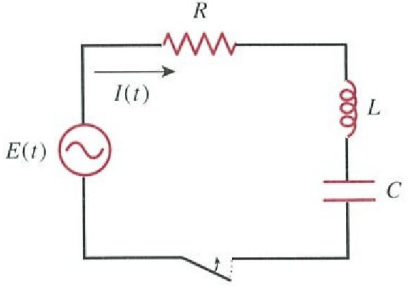
\includegraphics[]{figures/RLC.png}
    \caption{Basic RLC circuit}
\end{figure}

Using Kirchoff's law (KVL), the sum of drops is equal to the introduced voltage $E(t)$.

\begin{align}
    RI+L\dot I+\frac{q}{C}=E(t)\\
    R\dot q+L\ddot q+\frac{1}{C}q=E(t)
\end{align}

Thus, the auxiliary equation is

\begin{equation}
    Lm^2+Rm+\frac{1}{C}=0
\end{equation}

with solutions

\begin{equation}
    m=\frac{-R\pm \sqrt{R^2-\frac{4L}{C}}}{2L}\\
\end{equation}

Thus, the cases that arise are
\begin{itemize}
    \item \textbf{Damped Oscillatory}: $R^2-\frac{4L}{C}<0$
    \item \textbf{Critically Damped}: $R^2-\frac{4L}{C}>0$
    \item \textbf{Overdamped}: $R^2-\frac{4L}{C}>0$
\end{itemize}